\documentclass[tikz,border=2pt]{standalone}
\usepackage{amsmath,amssymb}
\usepackage{tikz}
\usetikzlibrary{arrows.meta}

\begin{document}
% Nonnegativity constraints x_1 >= 0, x_2 >= 0 restrict the choice variables to the closed
% positive quadrant; together with a resource constraint they cut out a triangle.
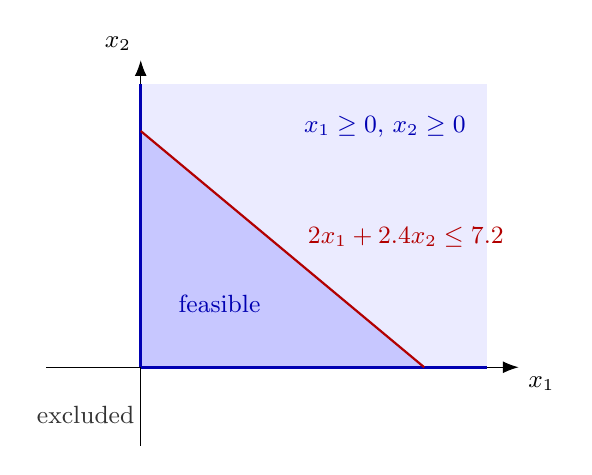
\begin{tikzpicture}[every node/.style={font=\small}, >={Latex[length=2mm]}]
	\fill[blue!8] (0,0) rectangle (4.4,3.6);
	\fill[blue!22] (0,0) -- (3.6,0) -- (0,3.0) -- cycle;
	\draw[->] (-1.2,0) -- (4.8,0) node[below right] {$x_1$};
	\draw[->] (0,-1.0) -- (0,3.9) node[above left] {$x_2$};
	\draw[blue!70!black, very thick] (0,0) -- (4.4,0);
	\draw[blue!70!black, very thick] (0,0) -- (0,3.6);
	\draw[red!70!black, thick] (3.6,0) -- (0,3.0);
	\node[red!70!black, anchor=west] at (2.0,1.65) {$2x_1+2.4x_2\le7.2$};
	\node[blue!70!black] at (3.1,3.05) {$x_1\ge0$, $x_2\ge0$};
	\node[blue!70!black] at (1.0,0.8) {feasible};
	\node[gray!40!black] at (-0.7,-0.6) {excluded};
\end{tikzpicture}
\end{document}
